\chapter[SM-ID of Continuous time systems]{Set-Membership identification of continuous time systems}

\begin{quotation}
    \noindent
    \textsf{In this chapter we are dealing with System Identification of continuous time systems. After an introduction to the problem in which we talk about identification in general, we move to the discussion about the identification of a continuous time model from noisy data (SM-Identification). Different approaches are analyzed including model transformation and Tustin discretization.}
\end{quotation}

\noindent
In this chapter we are considering the problem of estimating the parameters for a SISO LTI system described by a transfer function of the type:
\begin{equation}\label{eq:ct_model}
    H(s,\theta)=\frac{
        \beta_{n-1}{s^{n-1}}+\beta_{n-2}s^{n-2}+\dots+\beta_1{s}+\beta_0
    }{
        s^n+\alpha_{n-1}s^{n-1}+\alpha_{n-2}s^{n-2}+\dots+\alpha_1{s}+\alpha_0
    }
\end{equation}

\noindent
Where $\theta$ are the parameters of the system defined by:
\begin{equation}
    \theta=[\alpha_0\dots\alpha_{n-1},\beta_0,\dots,\beta_{n-1}]
\end{equation}
This problem must be solved by using \textbf{sampled} and \textbf{noisy} data. The experiment can be performed in the setup in \Cref{fig:CT_setup} in  by assuming that both input and output sampled data are affected by Unknown-but-bounded (UBB) noise.


\begin{multicols}{2}
    \begin{figure}[H]
        \centering 
        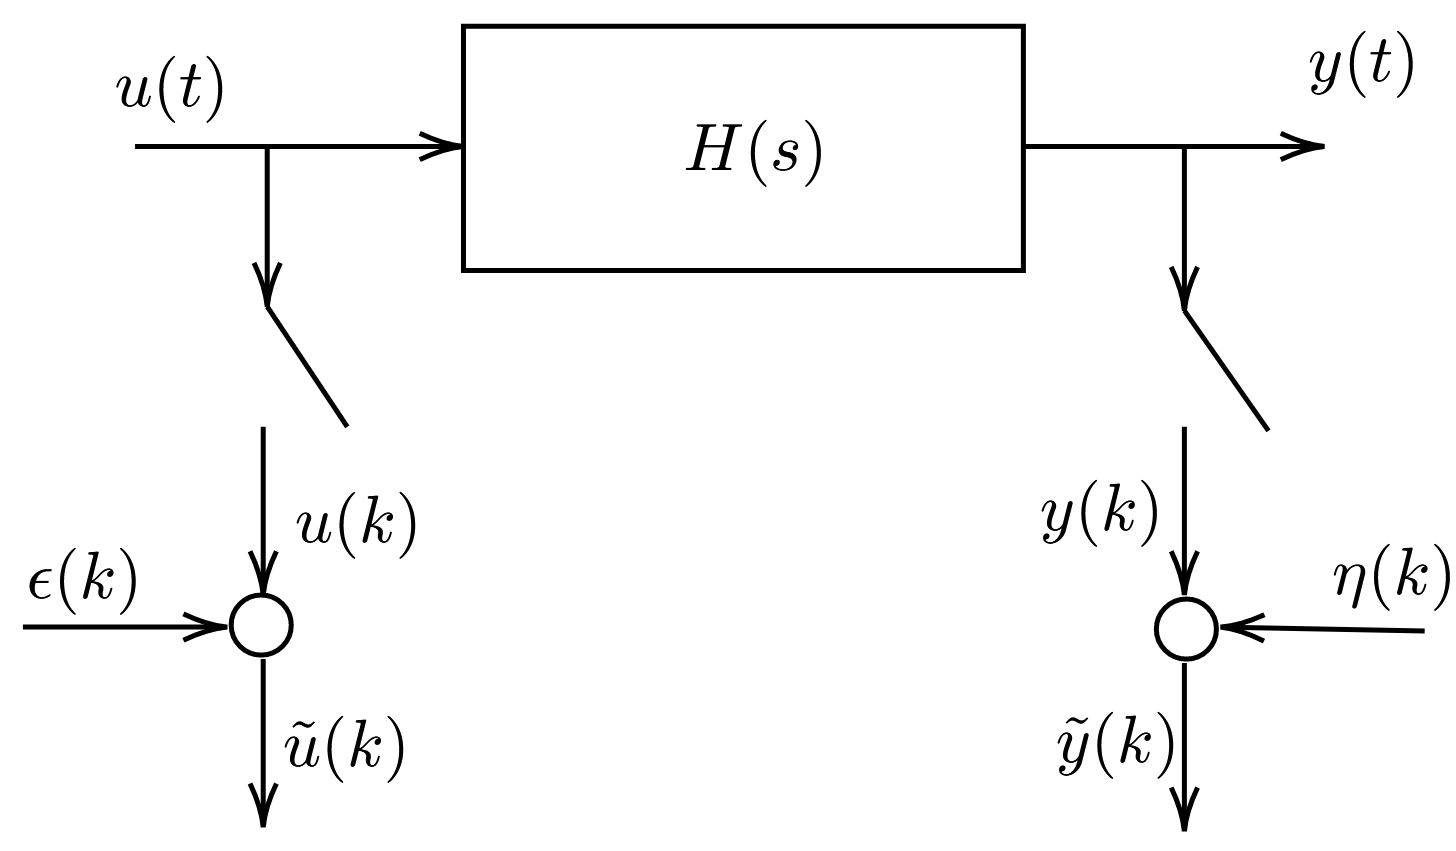
\includegraphics[scale=0.25]{img/CT_SM.png}
        \caption{SM-ID of SISO LTI CT system}
        \label{fig:CT_setup}
    \end{figure}
    Here we assume that:
    \begin{align*}
        y(k)=y(t=kT_s) \quad
        u(k)=y(t=k{T_s})
    \end{align*}
    The noise samples are such that 
    \begin{equation*}
        \vert \epsilon(k) \vert \le \Delta_\epsilon \quad
        \vert \eta(k) \vert \le \Delta_\eta
    \end{equation*}
\end{multicols}

\section{Motivations}
Here there are some motivations about the fact we could be interested in identifying a continuous time model. At first we can say that the parameters are not dependent on the sampling time, while in discrete time the smaller $T_s$ the higher is the probability to push all of the parameters toward 1\footnote{
    The mapping between s-plane and z-plane is dictated by the \textbf{sampling transformation}
    \begin{equation}
        z=e^{s{T_s}}
    \end{equation}  
    Here we have that for $T_s\to{0}$, $z\to1$
}. Moreover continuous time model are clonser to physical descriptions of physical systems. Finally the great majority of \textit{robust control techniques} (see $\mathcal{H}_\infty$, $\mu$-synthesis...) are in continuous time in their original formulation.

\section{Solution to the problem}
There are several approaches for solving the problem, each one of them having advantages and disadvantages. However, our main focus in on the set-membership approach to which we devote the great majority of this chapter.

\subsection{Indirect approach}
This is the case in which, first we estimate a discrete time model from noisy sampled data $\tilde{u}(k)$ and $\tilde{y}(k)$, then we use some discretization method to transform such a model into a continuous time one. This approach is very easy \underline{BUT}:
\begin{itemize}
    \itemsep-0.2em
    \item Does not solve the problem related to the parameters that goes to 1 with the decreasing sampling time $T_s$.
    \item Inverse discretization methods do not preserve important property of the identified system, first among the other, \textbf{stability}.
\end{itemize}
Anyway, we can use for example \textit{Least Squares} (taking care of all its disadvantages) and in \textsc{Matlab} the command \texttt{d2c} can be using with the objective of obtaining a continuous time transfer function.

\subsection{Direct approach}
In order to better understand the features and the issues raised up from such a \textbf{Direct approach}, we analyze an example.\\

\begin{figure}[h]
    \centering
    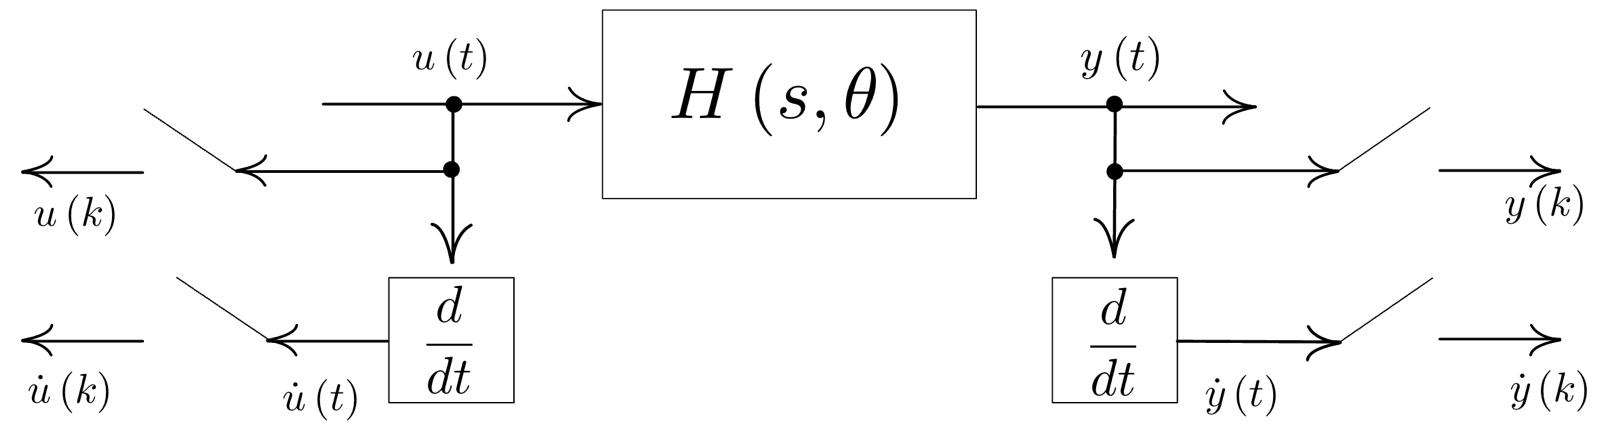
\includegraphics[scale=0.22]{img/derivators.jpg}
    \caption{Experimental settings using derivators}
\end{figure}
Suppose you want to identify the parameter of a model whose a-priori assumptions are saying us that the shape of its transfer function is 
\begin{equation}
    H(s)=\frac{\beta_0+\beta_1{s}}{s+\alpha_0}
\end{equation}
By applying the definition of transfer function relating the $\mathcal{L}$-transform of the input and the output, we can write down: 
\begin{equation}\label{eq:ex_laplace}
    y(s)=H(s)u(s) \iff 
    sy(s)+\alpha_0{y(s)}=\beta_1{s u(s)} + \beta_0 u(s)
\end{equation}
We want to go back in time domain (data are sampled in time) by inverse transforming the \Cref{eq:ex_laplace}, since we assume to start with a transfer function model, the initial conditions related to the input and the output are null. Then, in time domain we have 
\begin{equation}\label{eq:ex_time}
    \dot{y}(t)+\alpha_0{y(t)}=\beta_1\dot{u}(t)+\beta_0{u(t)}
\end{equation}

Note that if we sample the input and the output at $t=kT_s$ we can arrange the \Cref{eq:ex_time} in a matrix form, where the coefficient matrix contains the sample of $y(t), \ \dot{y}(t), \ u(t), \ \dot{u}(t)$, then we can use the Least-Squares to obtain the parameters with the assumption that the noise entering the data is modeled as a \textit{white gaussian noise}.
How can such samples be obtained? We can think to introduce some derivators in the experimental setting with the aim to sample the input/output of the system and its derivatives. However, there is a big problem: derivators are anticausal filters, though not phisically realizable!\\
Another idea could be the one of \textbf{estimating the derivatives} by introducing a sort of approximation in discrete time of the transfer function $H(s)=s$ representing a derivative in the Laplace domain. So we have that:
\begin{equation*}
    \dot{y}(k)\simeq D(q^{-1}) \tilde{y}(k) = D(q^{-1}) y(k) + D(q^{-1}) \eta(k)
\end{equation*}
Here we have to keep in mind that the sampled data are noisy! If such noise has high frequency components, this is hugely amplified, since $D{(q^{-1})}$ being an approximation of $s$ will have a shape similar to an \textit{High pass filter}. To conclude this discussion, if we had second derivatives, even worse. \\

%TODO: Add a figure here
In conclusion, also the idea to estimate the samples of the derivatives must be thrown out since even if the consistency property is perfectly fulfilled and data are noiseless, we have the non-negligible problem of the high pass filtering effect introduced by $D(q^{-1})$.

\subsection{System identification by using model transformation}
A possible way for going on about this topic is replacing the derivative operator $s$ with a low-pass filter of the type

\begin{equation}\label{eq:lambdat}
    \lambda(s)=\frac{1}{1+s\tau}
\end{equation}
Then, we want to estimate instead of $\dot{y}(t)$ and $\dot{u}(t)$ the following quantities based on such a type of \textit{model transformation}: 

\begin{equation}
    y^{(1)}(t)=\mathcal{L}^{-1}\{y^{(1)}(s)\}, \quad y^{(1)}(s)=\lambda(s)y(s)
\end{equation}

\noindent
By inverting the expression of \Cref{eq:lambdat}, we obtain another expression to substitute the Laplace variable $s$:

\begin{equation*}
    s=\frac{1-\lambda}{\lambda\tau}
\end{equation*}
Now, we obtain
\begin{align}
    &\frac{1-\lambda}{s\tau} y(s) + \alpha_0{y(s)}=\beta_1 {\frac{1-\lambda}{s\tau}} u(s) + \beta_0{u(s)}\\
    &y(s)-\lambda{y(s)}+\alpha_0\lambda\tau{y(s)}=\beta_1{u(s)}-\beta_1{\lambda}u(s)+\beta_0\lambda\tau{u(s)}\\
    &y(s)=(1-\alpha_0\tau)\lambda{y(s)} + \beta_1{u(s)}+(\beta_0\tau-\beta_1)\lambda{u(s)}\label{eq: last_step}
\end{align}

At this point we have to go back to \textit{time domain}. In particular the steps are the following:
\begin{enumerate}
    \itemsep-0.2em
    \item Substitute $\lambda$ with the \Cref{eq:lambdat}; 
    \item Compute the inverse Laplace transform $\mathcal{L}^{-1}$ 
\end{enumerate}
Doing such steps the \Cref{eq: last_step} becomes
\begin{equation}\label{eq:time_back}
    y(t)= \underbrace{(1-\alpha_0\tau)}_{\gamma_1} 
    y^{(1)}(t) + 
    \underbrace{\beta_1}_{\gamma_2} 
    {u(t)} 
    + \underbrace{(\beta_0\tau-\beta_1)}_{\gamma_3} u^{(1)}(t)
\end{equation}
where $\gamma_1$, $\gamma_2$, $\gamma_3$ are the parameters of the \textbf{transformed model}. You can arrange the \Cref{eq:time_back} in a matrix form by computing the function at time $t=kT_s$, $k=1,2,...$ and by using the Least-Squares the system can be (pseudo)inverted. The samples $y^{(1)}$ and $u^{(1)}$ can be obtained in simulation without amplifying the noise as in the case of an high pass filter approximating a derivator. The last step is obtaining the original parameters $\theta$ starting from the ones of the transformed model. Since
\begin{equation}
    \begin{cases}
        \gamma_1=1-\alpha_0t\\
        \gamma_2=\beta_1\\  
        \gamma_3=\beta_0\tau-\beta_1
    \end{cases} \iff \begin{bmatrix}
        \gamma_1\\\gamma_2\\\gamma_3
    \end{bmatrix}=\begin{bmatrix}
        -\tau&0&0\\
        0&0&1\\
        0&\tau&-1
    \end{bmatrix} \begin{bmatrix}
        \alpha_0\\
        \beta_0\\
        \beta_1
    \end{bmatrix}-\begin{bmatrix}
        1\\0\\0
    \end{bmatrix}=M\theta-v
\end{equation}
We can invert the system in order to retrieve from $\gamma$ the parameters $\theta$
\begin{equation}
    \theta = M^{-1}(\gamma-v)
\end{equation}

\section{Set-Membership identification}
Here the objective is to obtain a model for the system using noisy data and embedding the information on the noise directlty into the problem. As usual when you want to perform System Identification, we have to collect all of a-priori and a-posteriori information. 
\begin{enumerate}
    \item \textsc{A-priori information on the System} the system is continuous-time, described by the equation \Cref{eq:ct_model}; 
    \item \textsc{A-priori assumption on the noise} for sake of generality we assume that both input and output are affected by unkown but bounded noise $\epsilon(k)$ and $\eta(k)$, the bounds $\Delta_\eta$ and $\Delta_\epsilon$ are assumed to be known.
\end{enumerate}

At this point two approaches can be exploited in order to going on:
\begin{enumerate}
    \item \textsf{Model transformation}, this is not very used, however for further details you can consider the reference \citeauthor{johansson1994identification} \citetitle{johansson1994identification}, \citedate{johansson1994identification} \cite{johansson1994identification}; 
    \item \textsf{Tustin Discretization}, for this approach the main ideas are taken from \citeauthor{cerone2022set} \citetitle{cerone2022set}, \citedate{cerone2022set} \cite{cerone2022set}
\end{enumerate}

\subsection{Tustin discretization}
The \textit{Tustin discretization} is a \textbf{discretization method} than can be used when the function to be discretized has some regularity properties. The fundamental thing to be understand is: \textbf{what is the Tustin discretization of $1/s$}? In this way, after having retrieved such an expression a mapping between $z$ and $s$ using the Tustin method can be found. We know that given an integrator we have that its output can be computed as: 

\begin{multicols}{2}
    \begin{figure}[H]
        \centering
        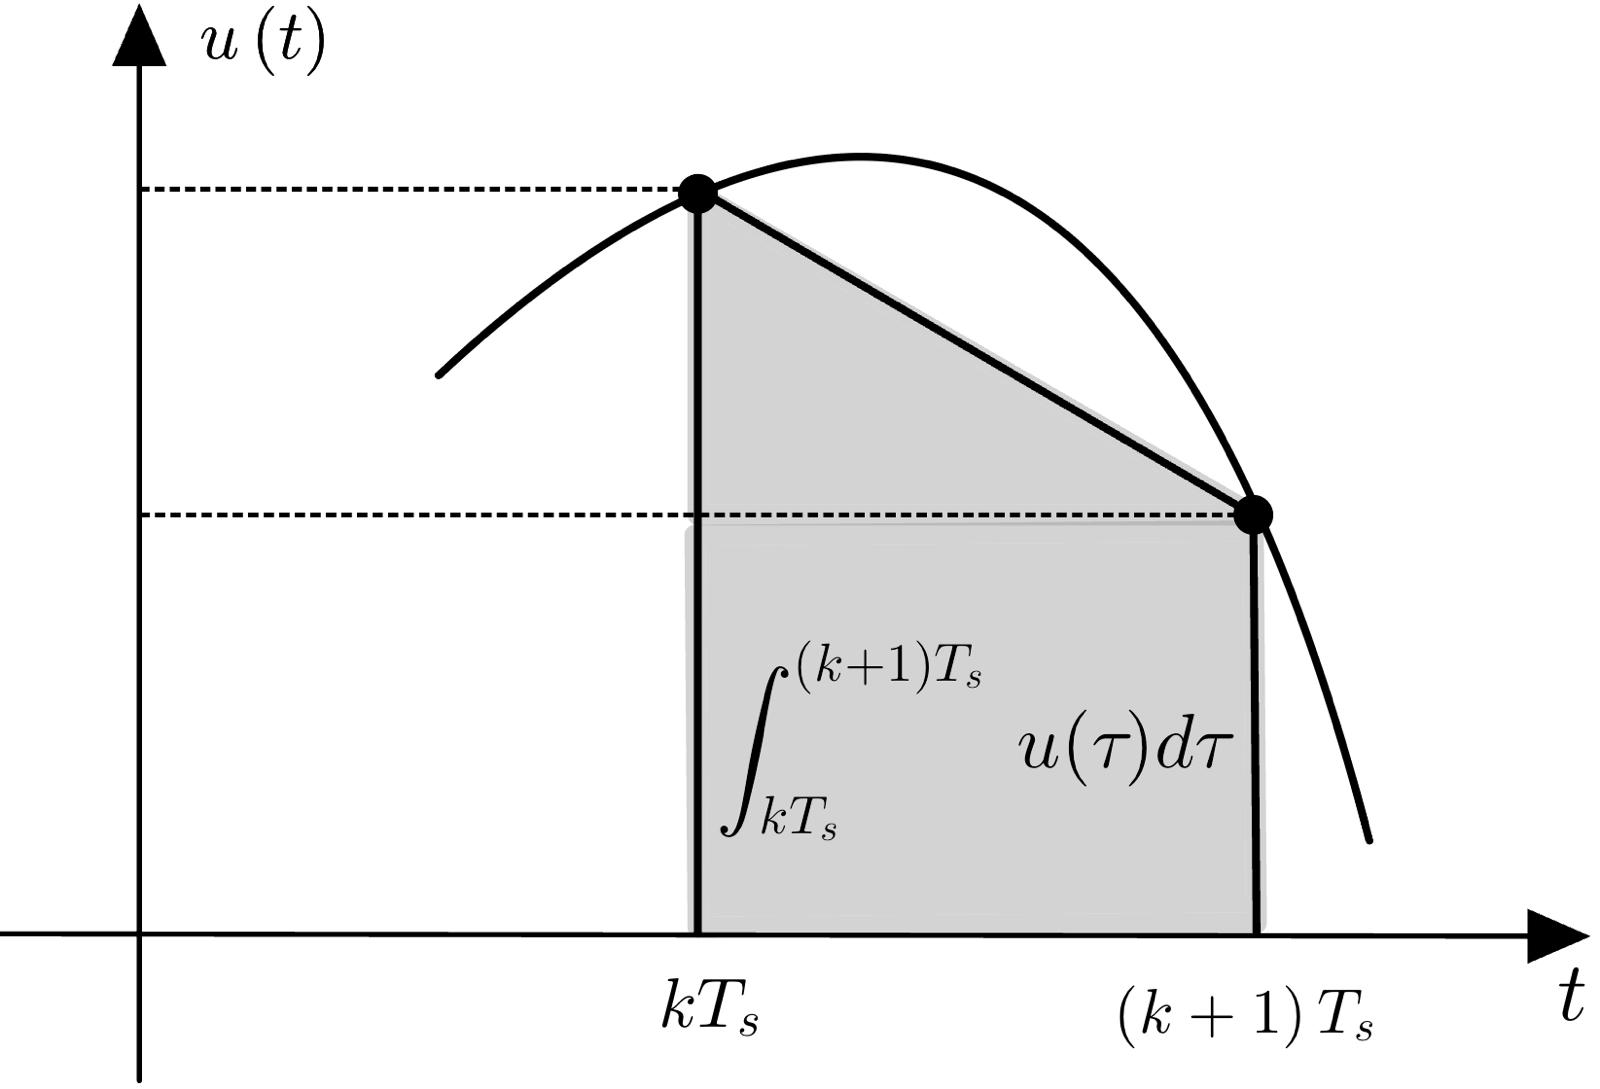
\includegraphics[scale=0.13]{img/Tustin_2.jpg}
        \caption{Idea behind Tustin Discretization}
    \end{figure}
    \begin{equation*}
        y(t)=y(t_0)+\int_{t_0}^t u(\tau){d\tau}
    \end{equation*}
    In the case of evaluating this expression at the instant $t=kT_s$ we have that 
    \begin{equation}
        y(k+1)=y(k)+\int_{kT_s}^{(k+1)T_s} u(\tau){d\tau}
    \end{equation}
\end{multicols}

\noindent
The second term of $y(k+1)$ is nothing but the area under the graph of $u(t)$. If we have  the assumption that the signal $u(t)$ has a shape such this area can be approximated by using a trapezoid, we can write that
\begin{equation}
    \int_{kT_s}^{(k+1)T_s} u(\tau){d\tau}=\frac{(u(k+1)+u(k))T_s}{2}
\end{equation}
which is the formula for computing the area of a trapezoid and $u(k)$, $u(k+1)$ are the basis, while $T_s$ (sampling time) is the height. Then we have:
\begin{align}
    &y(k+1)=y(k)+\frac{T_s}{2}(u(k+1)+u(k))\\
    &y(k+1)-y(k)=\frac{T_s}{2}(u(k+1)+u(k))\\
    &qy(k)-y(k)=\frac{T_s}{2}(qu(k)+u(k))\\
    &(q-1)y(k)=\frac{T_s}{2}(q+1)u(k) \iff 
    y(k)=\underbrace{\frac{T_s}{2}\frac{(q+1)}{(q-1)}}_{1/s}u(k)
\end{align}
Having the expression for  $1/s$ we can find that
\begin{equation}\label{eq:tustin_discret}
    s=\frac{2}{T_s}\frac{(z-1)}{(z+1)}
\end{equation}
where we have replaced the $q$ of the backward shift operator with $z$. Once we have such a discretization formula, you have to replace it the continuous time expression.

\subsection{Applying Tustin discretization to SM-ID}
As usual, is very effective giving an example by which we can discover the main properties of the approach of using the Tustin Discretization, the \Cref{fig:Tustin_1} shows the experimental settings. Suppose you have a continuous time model described by:
\begin{equation}\label{eq:ex_ct_model}
    H(s)=\frac{\beta_1{s}+\beta_0}{s^2+\alpha_1{s}+\alpha_0}
\end{equation}
By applying \Cref{eq:tustin_discret} the \Cref{eq:ex_ct_model} becomes a discrete time one discribed by:
\begin{equation}
    H(z)=\frac{
        {\beta_1{s\frac{2}{T_s}\frac{(z-1)}{(z+1)}}+\beta_0}
    }{
        \Big(\frac{2}{T_s}\frac{(z-1)}{(z+1)}\Big)^2+\alpha_1{\frac{2}{T_s}\frac{(z-1)}{(z+1)}}+\alpha_0
    }
\end{equation}
The output $y^{d}(k)$ of the model $H(z)$ when the sequence $u(k)$ is applied, in general is different than the sampled output of the real system $y(k)$ if all of the assumption are not fulfilled. More clearly:
\begin{align}
    &y(k)=y(t=kT_s), \ k=1,2,...\\
    &y^d{(k)}=H_{\text{Tustin}}(q^{-1})u(k)\\
    &\delta(k)=y^d(k)-y(k)
\end{align}
where $\delta(k)$ denotes the gap between the two sequences for each $k$ and so it plays the role of a \textbf{discretization error}. By assumption we assume that such a difference is bounded by a constant $\Delta_\delta$ assumed to be known.\\
 Since, we measure the output affected by noise, we can write that
\begin{equation}
    \delta(k)=y^d(k)-\tilde{y}(k)+\eta(k) \iff 
    \delta(k)-\eta(k)=\eta'(k)=y^d(k)-\tilde{y}(k)
\end{equation}
Since we know also the bound for $\eta$ we have that 
\begin{equation}
    \vert \eta'(k) \vert \le \Delta_\eta+\Delta_\delta
\end{equation}

\begin{figure}
    \centering
    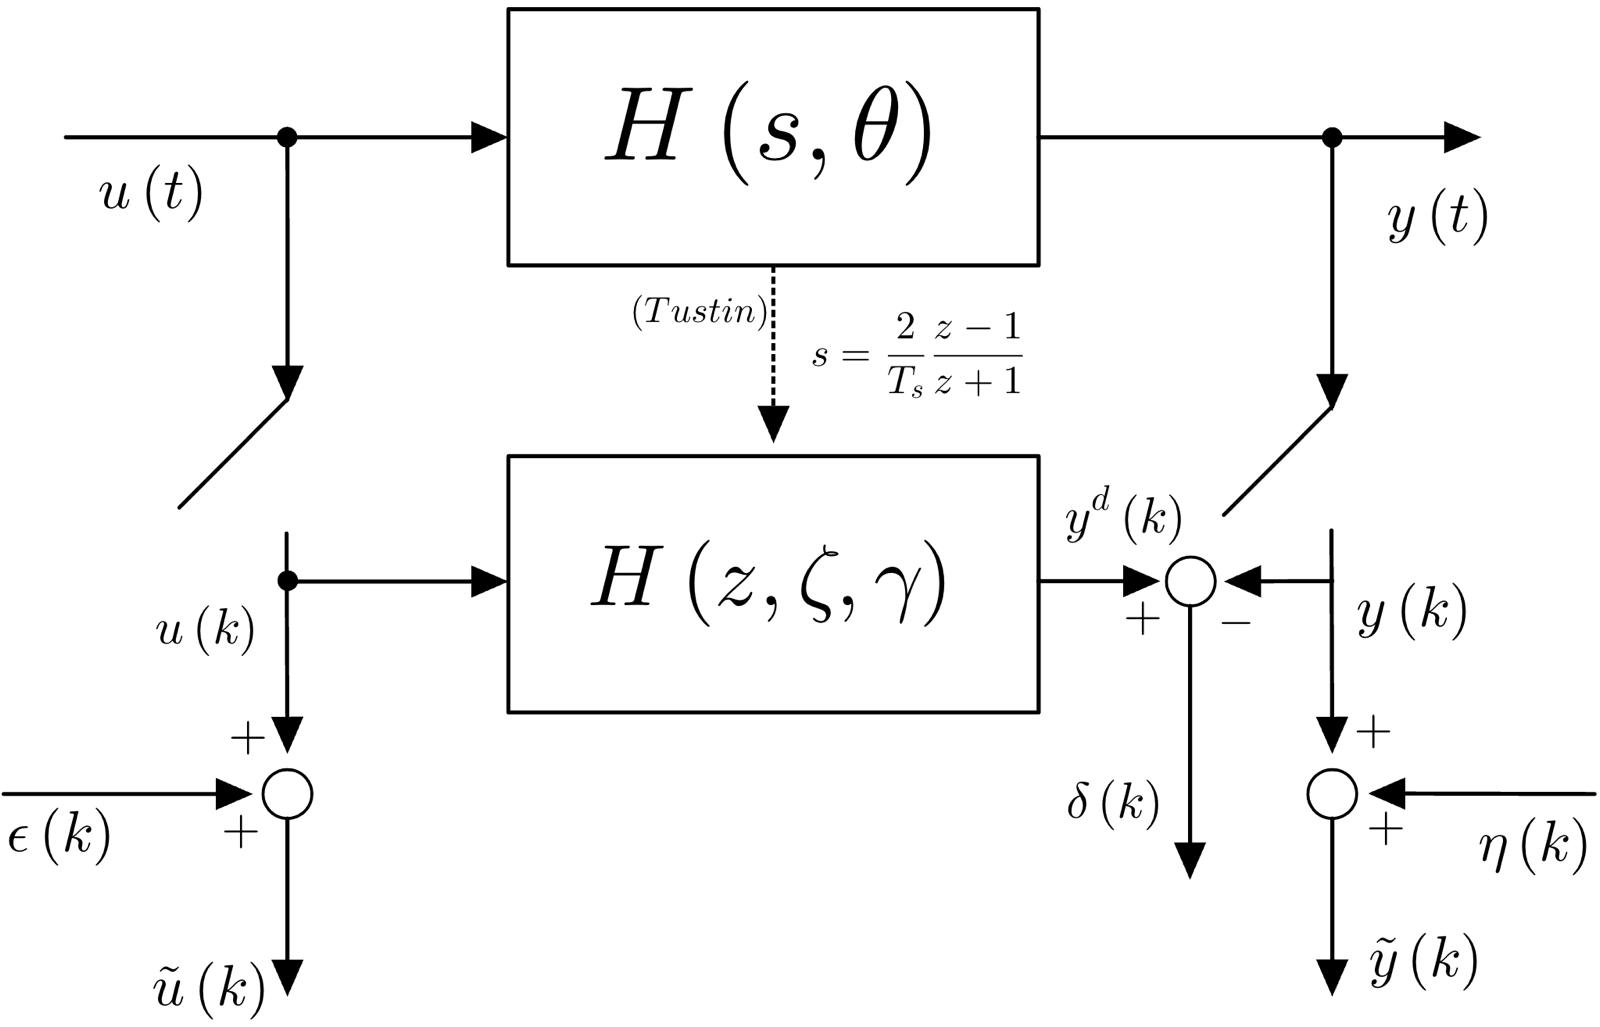
\includegraphics[scale=0.21]{img/Tustin.jpg}
    \caption{Tustin disretization experimental settings}
    \label{fig:Tustin_1}
\end{figure}

Now we can define the feasible parameter set by putting together all of the a-priori and a-posteriori information:
\begin{equation}
    \begin{aligned}
        \mathcal{D}_{\theta}=&\big\{\theta\in\mathbb{R}^4: 
            \ y(t)=H(s,\theta)u(t) \\
            &H(z)=\frac{
        {\beta_1{s\frac{2}{T_s}\frac{(z-1)}{(z+1)}}+\beta_0}
    }{
        \Big(\frac{2}{T_s}\frac{(z-1)}{(z+1)}\Big)^2+\alpha_1{\frac{2}{T_s}\frac{(z-1)}{(z+1)}}+\alpha_0
    }\\ 
        &\tilde{y}(k)=y^d(k)+\eta'(k), \quad  \vert \eta'(k) \vert \le \Delta_\eta+\Delta_\delta\\
        &\tilde{u}(k)=u(k)+\epsilon(k) \quad y^d(k)=H(z)u(k) \quad k=1,...,N
        \big\}
    \end{aligned}
\end{equation}
\noindent
We know that such a set $\mathcal{D}_{\theta}$ must be extended, but it is the case to rewrite $H(z)$ in a more compact form, in particular if we do all the algebraic steps are needed at the end we obtain:
\begin{equation}
    H(z)=\frac{
        z^2 \overbrace{[2T_s\beta_1+T_s \beta_0]}^{b_2(\beta)}+
        z \overbrace{{[2T_s\beta_0]}}^{b_1(\beta)}+ 
        \overbrace{T_s^2\beta_0-2T_s\beta_1}^{b_0(\beta)}}
        {
            z^2\underbrace{[4+2\alpha_1T_s+T_s^2\alpha_0]}_{a_2(\alpha)}+
            z \underbrace{[2T_s^2\alpha_0-8]}_{a_1(\alpha)}+
            \underbrace{4-2\alpha_1T_s+T_s^2\alpha_0}_{a_0(\alpha)}
        }
\end{equation}

\noindent
We want that the denominator being a \textit{monic} polynomial (the leading coefficient equal to 1)\footnote{
    Allowing a "no-one" leading coefficient we are allowing arbitrary rescaling of all the coefficient, achieving  bad-posedness of the  problem.
}, so that at the end of the  day we can write:
\begin{equation}
    H(z,\zeta,\gamma)=\frac{\zeta_2z^2+\zeta_1{z}+\zeta_0}{z^2+\gamma_1{z}+\gamma_0}
\end{equation}
\noindent
The new parameters $\zeta, \gamma$ are such that
\begin{equation}
    \begin{aligned}
        &\zeta_2=\frac{b_2(\beta)}{a_2(\alpha)}\quad 
        \zeta_1=\frac{b_1(\beta)}{a_2(\alpha)}\quad
        \zeta_0=\frac{b_0(\beta)}{a_2(\alpha)}\qquad
        \gamma_1=\frac{a_1(\alpha)}{a_2(\alpha)} \quad
        \gamma_0=\frac{a_0(\alpha)}{a_2(\alpha)}\quad
    \end{aligned}
\end{equation}
These new additive (slack) optimization variable are dependent on the parameters $\theta=[\alpha, \beta]^T$ and results in bilinear constraints on the optimization variables, they must be embedded in the description of the \textit{extended feasible parameter set}:
\begin{equation}
    \begin{aligned}
        \mathcal{D}_{\theta,\zeta,\gamma,\epsilon,\eta'}=&\big\{
            (\theta,\zeta,\gamma,\epsilon,\eta')\in\mathbb{R}^{n_\theta+5+2N}:\\
            &  \vert \eta'(k) \vert \le \Delta_\eta+\Delta_\delta \quad
            \vert \epsilon(k) \vert \le \Delta_\epsilon \ k=1,...,N\\
        &\tilde{u}(k)=u(k)+\epsilon(k) \quad k=1,...,N\\
        %&y^d(k)=H(q^{-1},\zeta,\gamma)u(k) \quad 
        %k=n+1,...,N\\
        %&y^d(k)+\gamma_1{y^d(k-1)}+\gamma_0{y^d(k-2)}=
        %\zeta_2u(k)+\zeta_1{u(k-1)}+\zeta_0{u(k-2)}\\
        &\tilde{y}(k)-\eta'(k)+\gamma_1{\tilde{y}(k-1)-\gamma_1\eta'(k-1)+\gamma_2{\tilde{y}(k-2)}+\gamma_2\eta'(k-2)}=\\
        &=\zeta_2\tilde{u}(k)-\zeta_2\epsilon(k)+\zeta_1\tilde{u}(k-1)-\zeta_1\epsilon(k-1)+\zeta_0\tilde{u}(k-2)-\zeta_0\epsilon(k-2) \ \ k=n+1,...,N\\
        &
        \underbrace{\zeta_i a_2(\alpha)=b_i(\beta) \quad i=0,1,2   \quad \gamma_i a_2(\alpha)=a_i(\alpha)}_{\textsf{bilinear in}\  \theta,\zeta,\gamma \quad i=0,1}
    \big\}
    \end{aligned}
\end{equation}
The problem of computing the PUI on $\alpha, \beta$ is a POP of degree 2 (can be solved by SparsePOP). The optimization problems to be solved are 
\begin{equation}
    \underline{\theta}_i=\min_{(\theta,\zeta,\gamma,\epsilon,\eta')\in\mathcal{D}_{\theta,\zeta,\gamma,\epsilon,\eta'}} \theta_i, \quad \overline{\theta_i}=\max_{(\theta,\zeta,\gamma,\epsilon,\eta')\in\mathcal{D}_{\theta,\zeta,\gamma,\epsilon,\eta'}} \theta_i, \qquad 
    PUI_i=[\underline{\theta}_i \ \overline{\theta}_i ]
\end{equation}

\begin{remark}
    If we assume that $\Delta_\delta=0$ and we use \textbf{noise free} data, then the problem of finding the PUIs is \textbf{infeasible}, since even if we are using data not being corrupted by noise we are assuming that there is bounded noise on both input and output. Moreover we are saying that we are in the ideal condition in which between one point and the other there is a \textbf{straigth line}.
\end{remark}

\begin{remark}
    Notice that the bound on the discretizationn error, must be provided as an \textit{a-priori assumption}, however it depends on $T_s$ and $u(t)$.
\end{remark}

From these two remarks we can say that the information $\Delta_\delta$ cannot be neglected otherwise we have infeasibility. So a common way to go beyond such a problem is to find \textbf{the minimal value for $\Delta_\delta$ such that the problem has at least a solution}. We have to solve an optimization problem over the same feasible parameter set, with the only difference that the bound on the discretization error is an optimization variable.

\subsection{Estimating $\Delta_\delta$ from data}
There is the possibility to estimate the bound $\Delta_\delta$ on the discretization error, however there is no guarantee that we are not adding conservativeness. Anyway the way of proceeding is the following:
\begin{equation}
    \begin{aligned}
        \Delta_\delta^*&=\min_{(\Delta_\delta,\theta,\zeta,\gamma,\epsilon,\eta')\in\mathcal{D}_{\Delta_\delta,\theta,\zeta,\gamma,\epsilon,\eta'}} \Delta_\delta\\
        &\text{s.t.} \\
        &\tilde{y}(k)=y^d(k)+\eta'(k) \quad 
          \vert \eta'(k) \vert \le \Delta_\eta+\Delta_\delta \quad
        \vert \epsilon(k) \vert \le \Delta_\epsilon \ k=1,...,N\\
    &\tilde{u}(k)=u(k)+\epsilon(k) \quad k=1,...,N\\
    %&y^d(k)=H(q^{-1},\zeta,\gamma)u(k) \quad 
    %k=n+1,...,N\\
    %&y^d(k)+\gamma_1{y^d(k-1)}+\gamma_0{y^d(k-2)}=
    %\zeta_2u(k)+\zeta_1{u(k-1)}+\zeta_0{u(k-2)}\\
    &y^d(k)=H(q^{-1},\zeta,\gamma)u(k) \quad 
    k=n+1,...,N\\
    &
    \zeta_i a_2(\alpha)=b_i(\beta) \quad i=0,1,2   \quad \gamma_i a_2(\alpha)=a_i(\alpha) \quad i=0,1
    \end{aligned}
\end{equation}

\section*{References}
\begin{itemize}
    \itemsep-0.3em
    \item[\Large{\ding{45}}]  \Citeauthor{johansson1994identification}, \textit{\citetitle{johansson1994identification}}, \citedate{johansson1994identification}
    \item[\Large{\ding{45}}]  \Citeauthor{cerone2022set}, \textit{\citetitle{cerone2022set}}, \citedate{cerone2022set}
\end{itemize}